\section{What is HSkAnner3D?}
    \begin{figure}[H]
        \centerline{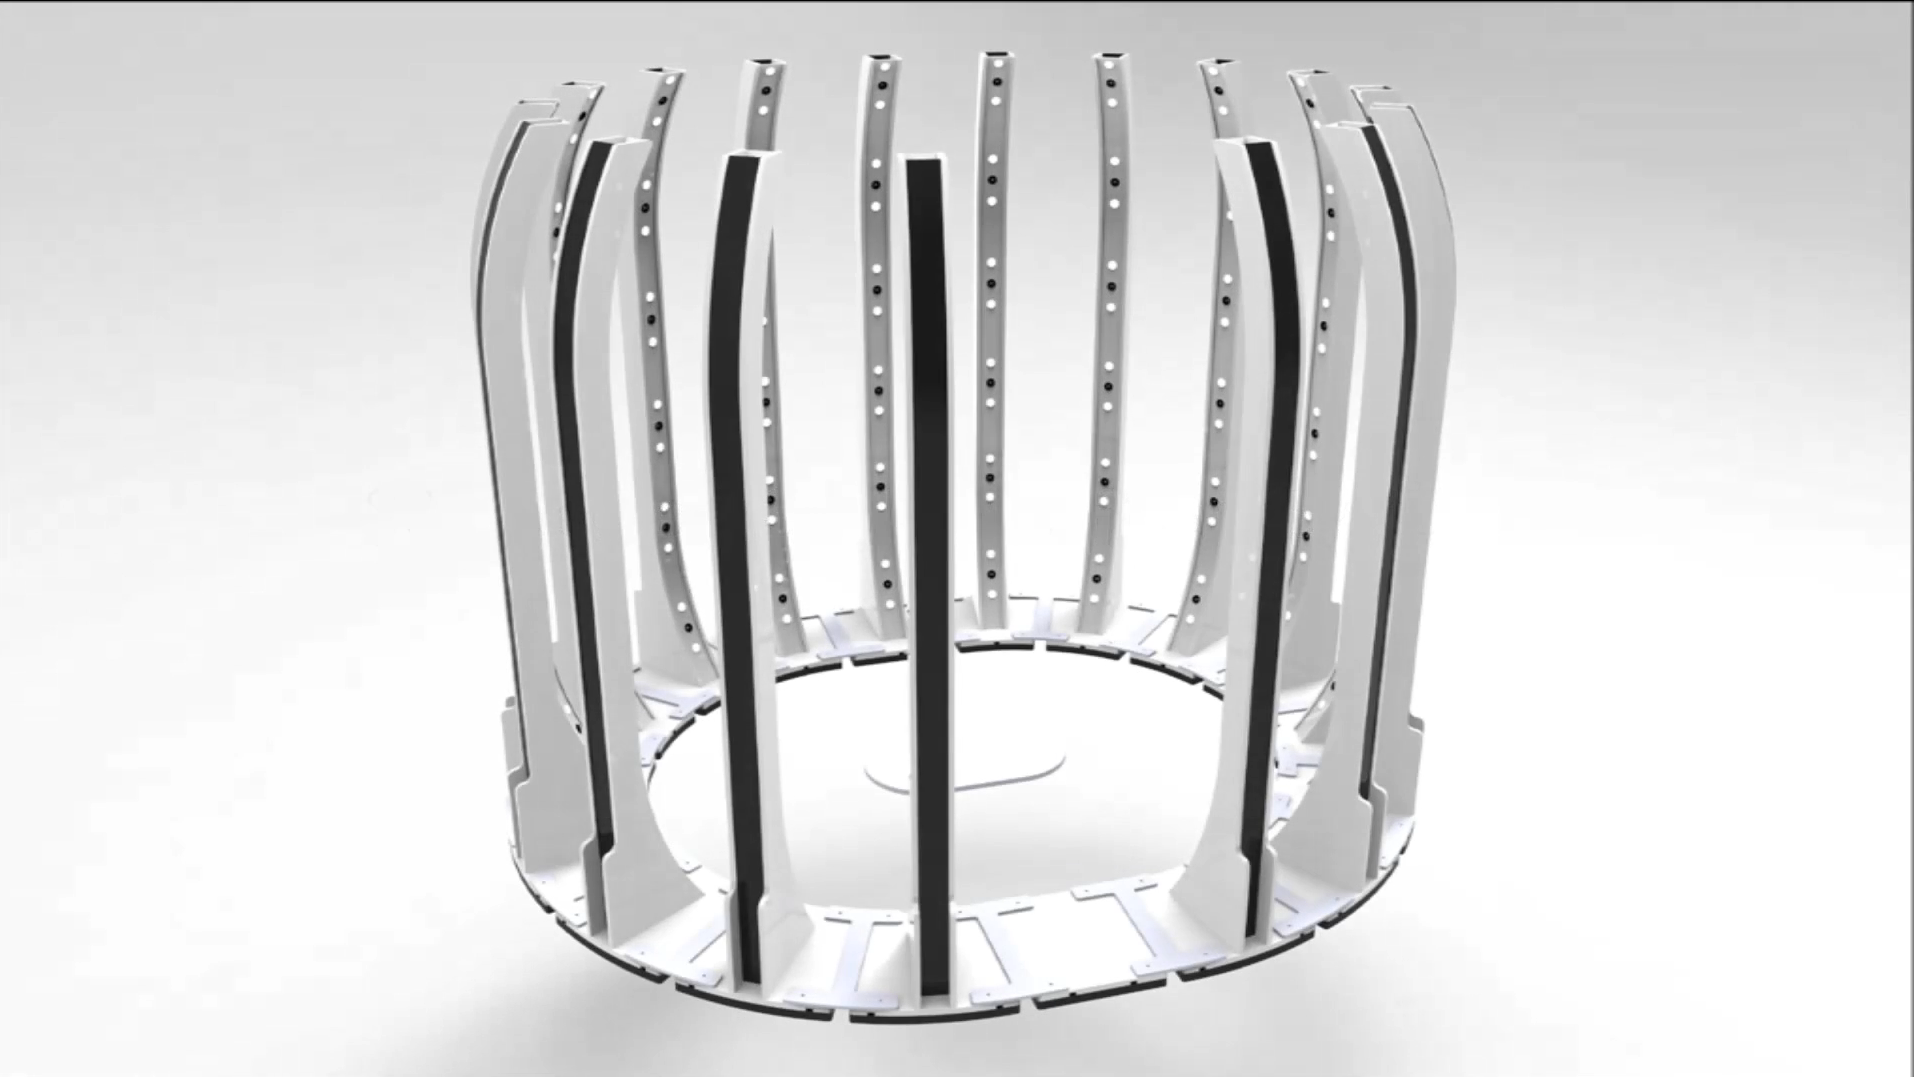
\includegraphics[width=\linewidth]{what/korean_scanner.png}}
        \caption{A similar physical approach to this one by MakeShape \cite{scanner_korean} will be taken for the array}
    \label{korean}
    \end{figure}

    HSkAnner3D is
    \begin{itemize}
        \item a 3D scanner $\xrightarrow[]{}$ creates 3D models from 3D objects placed in the scanning space - the goal is to be able to do full body scans of humans
        \item a local system $\xrightarrow[]{}$ no external dependencies, just mains power
        \item easy to use $\xrightarrow[]{}$ can be operated by just about everyone
    \end{itemize}
    
    It uses
    \begin{itemize}
        \item an array of lights, controlled by lighting controllers $\xrightarrow[]{}$ to illuminate the subject
        \item an array of cameras, each controlled by a single board computer (SBC) $\xrightarrow[]{}$ to capture 2D color images of the subject from many different angles
        \item a powerful computer $\xrightarrow[]{}$ to calculate 3D models from a set of 2D images using photogrammetry software and for controlling the arrays
        \item network cables and a network switch $\xrightarrow[]{}$ to connect the SBCs and lighting controllers to the computer
    \end{itemize}
    
\section{System Architecture}
    \begin{figure}[H]
        \centerline{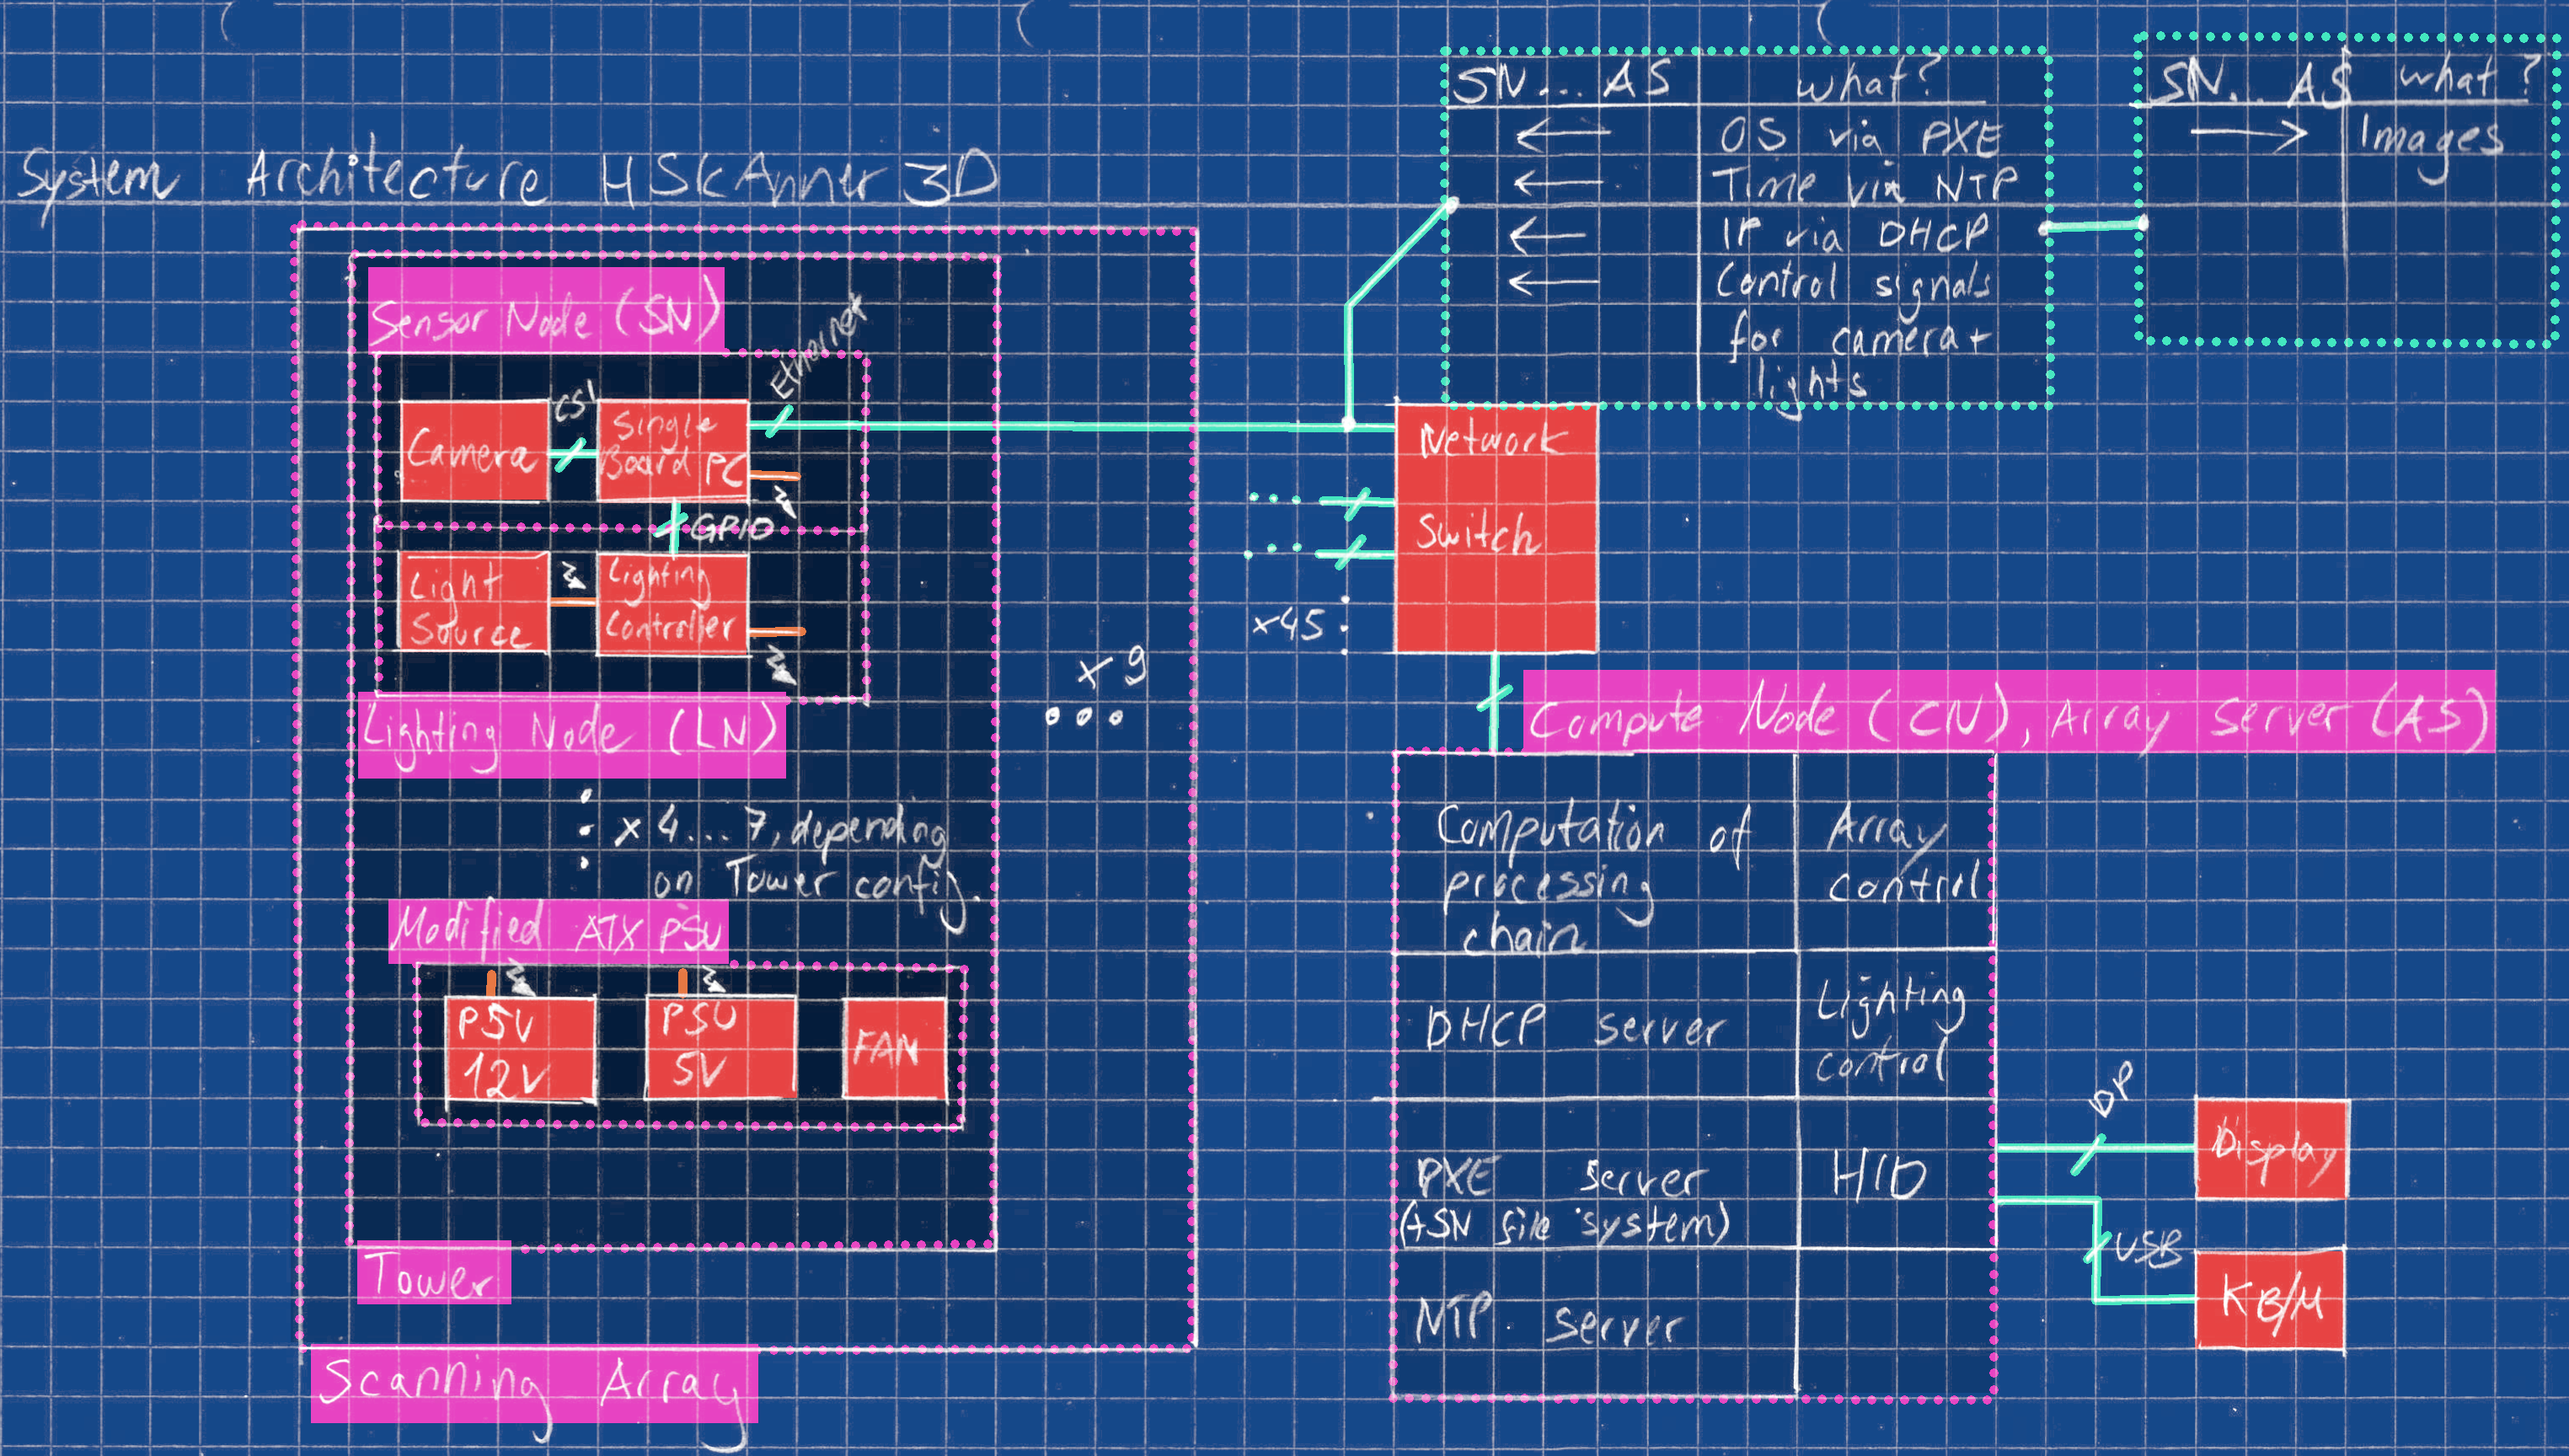
\includegraphics[width=\linewidth]{what/sysarch-system.png}}
        \caption{Preliminary architecture of the scanning system. \newline
	        \textbf{Legend}\newline
	        \textit{Pink} Building block \newline
	        \textit{Red} Hardware component \newline
	        \textit{Cyan} Data (line) \newline
        		\textit{Orange} DC power
        }
    \label{sysarch-system}
    \end{figure}
    
    Note: I am aware that there are adapters to use two cameras with one Raspberry Pi. But I have done some research and it seems like the reliablity of those is not very high, thus they are not suitable for this project.
    
\section{Why is it necessary to build HSkAnner3D?}
	Hochschule Karlsruhe does currently not have a 3D scanner, so it's missing out on the core features of such a system:
	\begin{itemize}
		\item being able to recreate complex shapes in 3D space without much effort
		\item creating 3D video data for use with e.g. motion tracking (will only be implemented if I have the time)
	\end{itemize}

	There is a plethora of arguments for building your own scanning system over buying a finished product:
	\begin{itemize}
		\item Cost \newline
			Commercial solutions like the one MakeShape is offering cost large amounts of money. Their scanner uses $100$ cameras, but costs around $43 000$\euro{}. HSkAnner3D has a total project budget of $5 000$\euro{} (including research \& development cost). Cost is also the reason why HSkAnner3D uses photogrammetry as a technique to generate 3D data, since depth cameras are very expensive.
		\item Flexibility \newline
			Since all parts of the system, be it hardware or software, are designed to be modular, interchangable and adjustable, the system can be altered at will to suit different needs in the future.
		\item Easy maintenance \newline
			The modularity helps make the system be more easily maintainable. The hardware and software is written and assembled with repairabilty in mind.
		\item Well documented \newline
			As the project is developed in-house, there's no secret sauce. All code and design assets are available for future improvements and enhancements by students of the Hochschule.
	\end{itemize}

\section{How does HSkAnner3D work? The operation principle of the system}
    \begin{figure}[H]
        \centerline{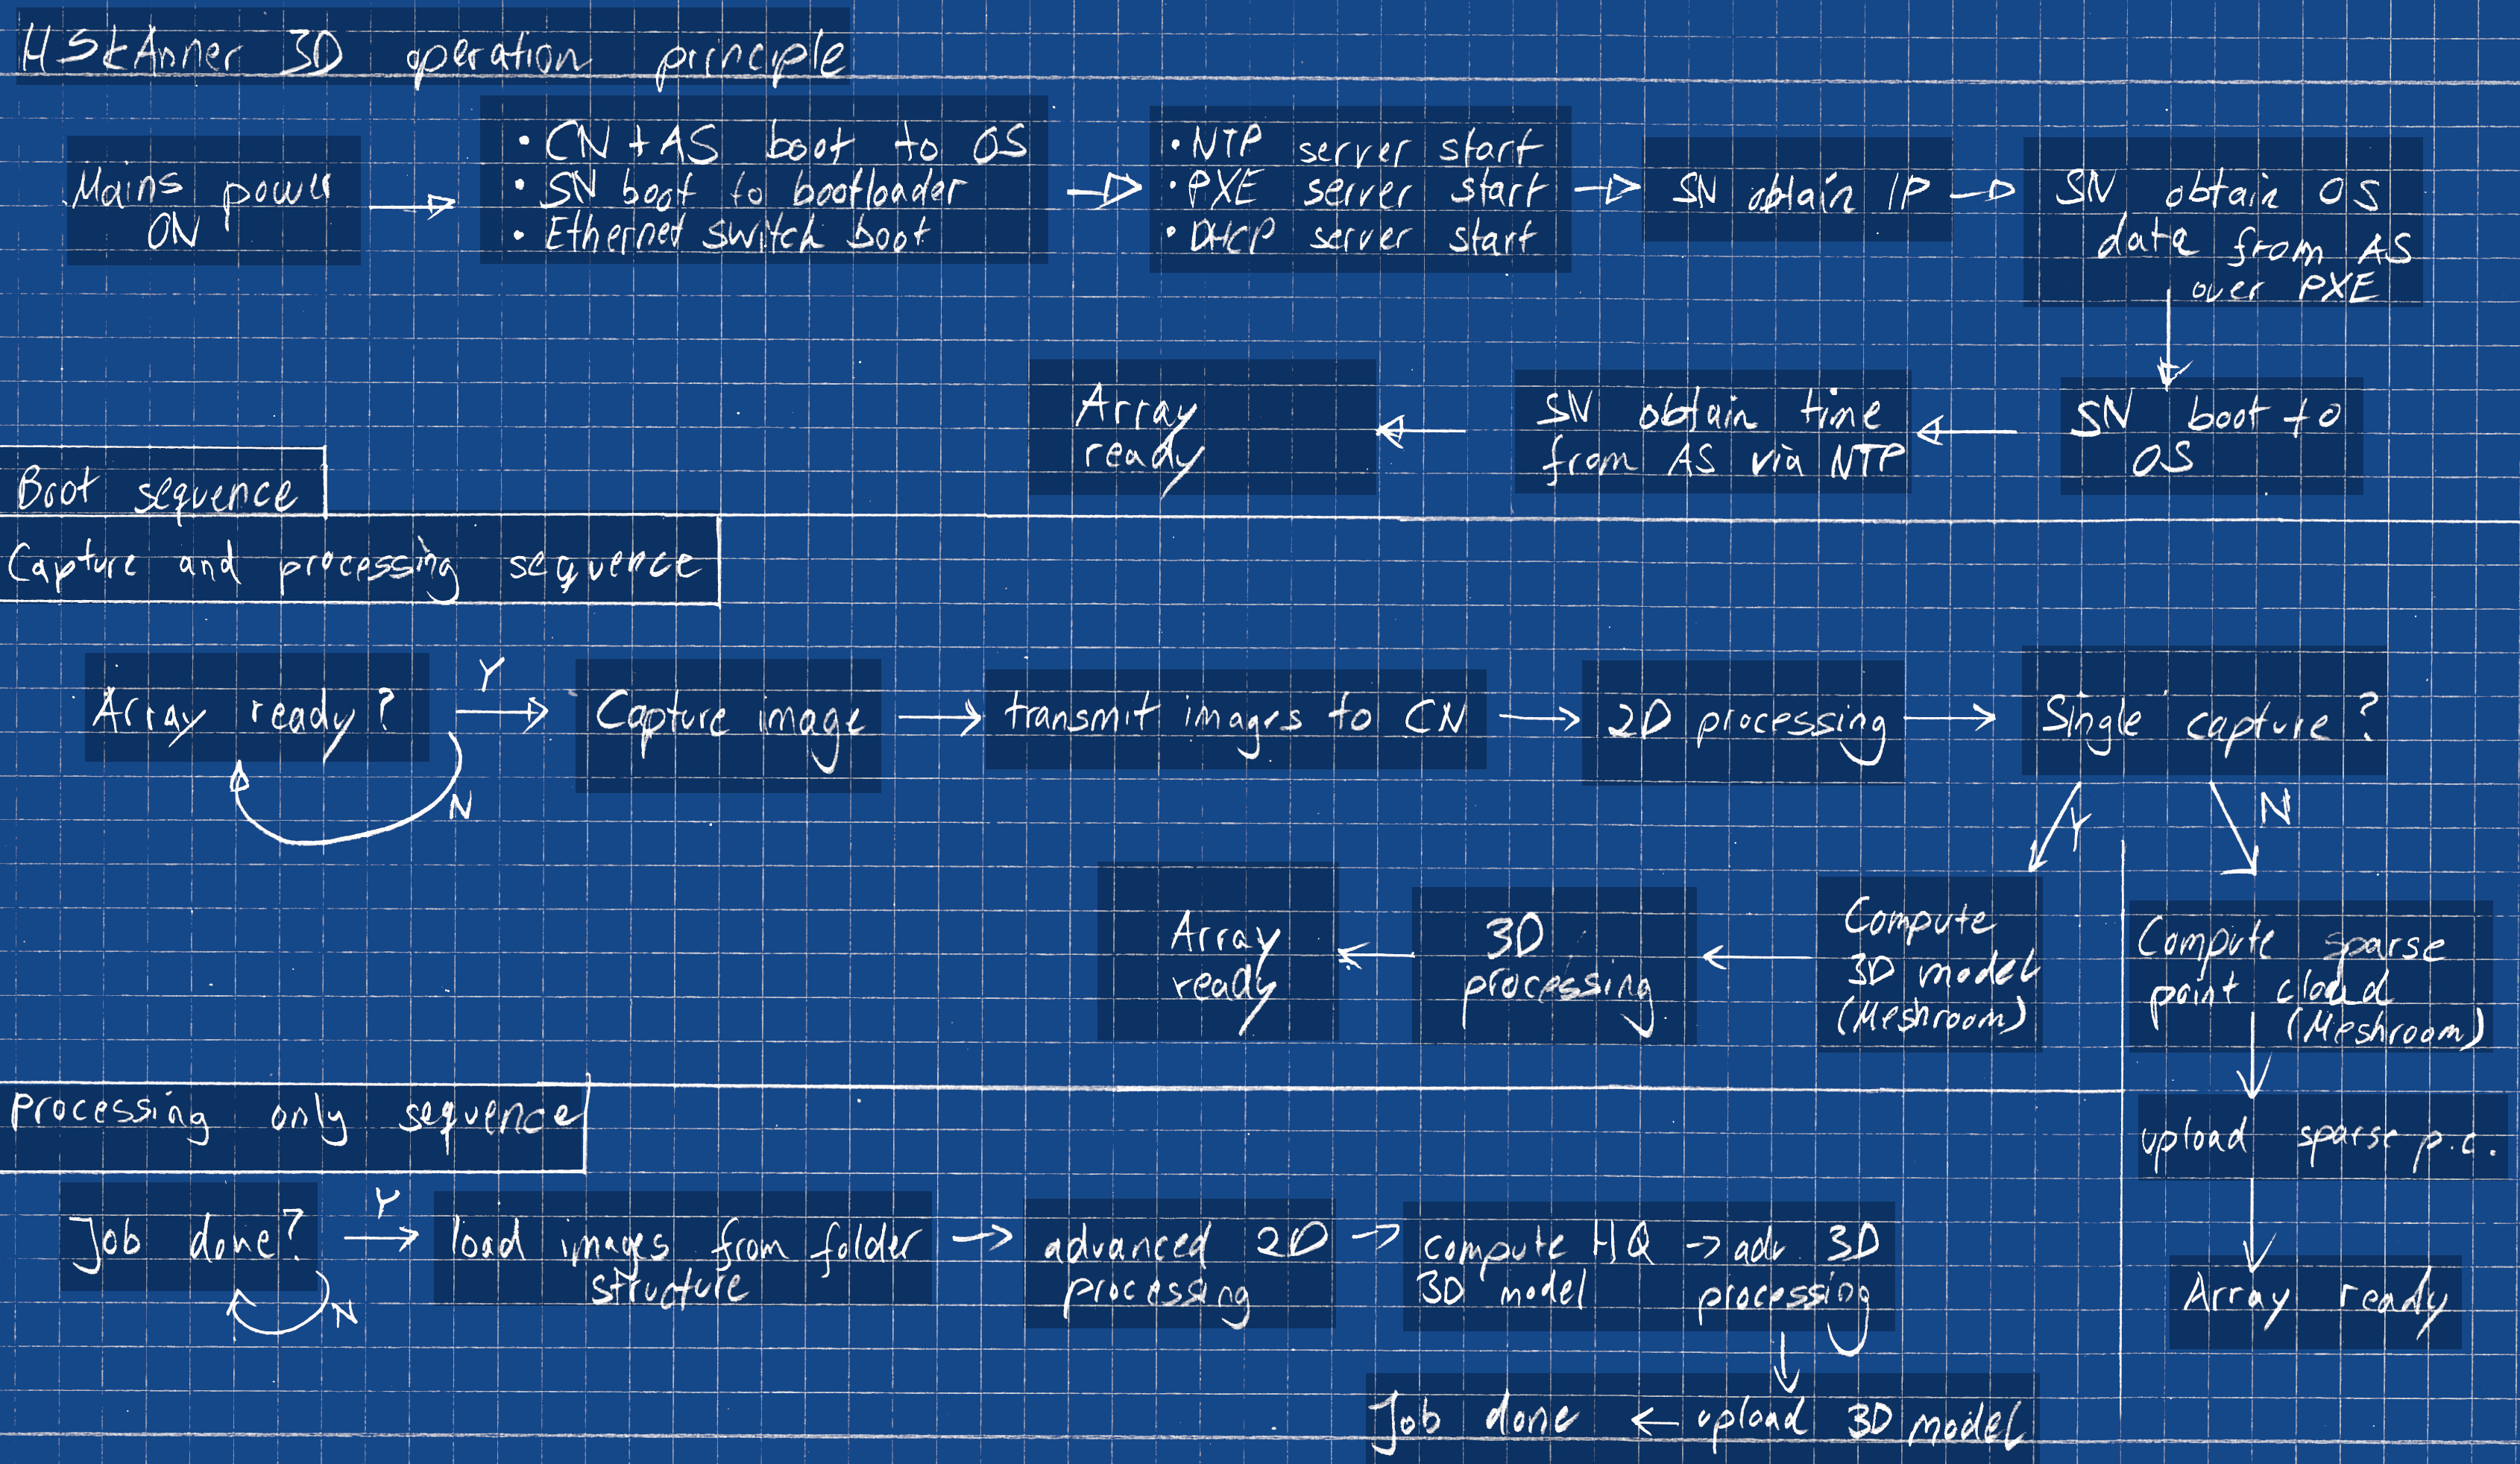
\includegraphics[width=\linewidth]{what/processing-chain-system.png}}
        \caption{HSkAnner3D working principle flowchart}
    \label{operation-flowchart-system}
    \end{figure}
